\subsection{Performance Comparison on High-Dimensional Benchmarks}
\label{sec:exp_highdim}

\begin{table*}[!t]
\centering
\begin{threeparttable}
\caption{Macro-Precision (\%) on High-Dimensional Benchmarks ($K = \lfloor 0.15p \rfloor$, $B = 1{,}000$)}
\label{tab:highdim_wide}
\scriptsize
\setlength{\tabcolsep}{7.0pt}
\renewcommand{\arraystretch}{1.06}
\begin{tabular}{@{}lrrrrrrrrr@{}}
\toprule
Dataset & GA & BPSO & EDA & MEL & mRMR & ReliefF & L1-LR & RF-Imp & SP-PD \\
\midrule
arcene                    & 80.73 & 83.00 & 79.74 & 75.70 & 81.26 & \textbf{83.59} & 77.81 & 80.85 & 80.80 \\
Gutenberg                 & 57.66 & 68.46 & 68.41 & 67.08 & \textbf{73.13} & 58.34 & 61.96 & 63.20 & 71.91 \\
DrivFace                  & \textbf{93.24} & 91.92 & 89.51 & 90.55 & 89.05 & 89.89 & 86.87 & 88.55 & 91.94 \\
DLBCL/Lymphoma\tnote{a} & 76.24 & 76.74 & 80.72 & 81.61 & 80.26 & 81.46 & 81.25 & 80.20 & \textbf{85.73} \\
relathe                   & 79.34 & 80.32 & 80.99 & 81.97 & 79.85 & 78.93 & 82.68 & 79.14 & \textbf{84.19} \\
lung                      & 88.21 & 94.10 & 86.80 & \textbf{96.48} & 93.83 & 95.91 & 94.92 & 92.44 & 91.71 \\
warpPIE10P                & 90.61 & 87.70 & 87.72 & 92.06 & 95.88 & \textbf{96.53} & 94.93 & 93.08 & 94.51 \\
malware                   & 97.20 & 98.23 & 98.23 & \textbf{98.61} & 87.59 & 94.61 & 95.61 & 94.61 & 97.17 \\
COIL20                    & 97.73 & 97.35 & \textbf{98.57} & 97.93 & 96.31 & 96.85 & 97.74 & 97.49 & 97.44 \\
ORL                       & 82.44 & 85.45 & 84.20 & 83.85 & 84.74 & 78.24 & \textbf{86.66} & 83.67 & 83.32 \\
CNAE-9                    & 87.03 & 84.91 & \textbf{89.40} & 85.91 & 88.48 & 84.64 & 86.91 & 85.43 & 88.86 \\
isolet                    & 83.98 & 83.66 & 87.25 & 87.29 & 82.08 & 77.37 & 86.85 & 85.13 & \textbf{87.92} \\
madelon                   & 81.50 & 83.81 & 86.64 & 83.31 & 80.03 & 83.48 & 56.21 & 84.18 & \textbf{88.29} \\
\midrule
Mean                      & 84.30 & 85.82 & 86.01 & 86.33 & 85.58 & 84.60 & 83.88 & 85.23 & \textbf{87.98} \\
Mean \#Feat               & 458.3 & 492.5 & 503.0 & 302.9 & 513.9 & 513.9 & 299.1 & 513.9 & \textbf{200.1} \\
Friedman Rank             & 6.15 & 4.96 & 4.35 & 4.00 & 5.38 & 5.92 & 4.92 & 5.92 & \textbf{3.38} \\
$p$-value\tnote{b}        & 0.008 & 0.057 & 0.033 & 0.057 & 0.147 & 0.022 & 0.080 & 0.011 & -- \\
\bottomrule
\end{tabular}
\begin{tablenotes}[flushleft]
\scriptsize
\item[a] Averaged over DLBCL and lymphoma as one independent group.
\item[b] Two-sided Wilcoxon signed-rank $p$-values comparing SP-PD with each baseline across the 13 groups.
\end{tablenotes}
\end{threeparttable}
\end{table*}


Table~\ref{tab:highdim_wide} compares macro-precision across the 13 high-dimensional groups at $K = \lfloor 0.15p \rfloor$ and $B = 1{,}000$. SP-PD achieves the highest mean macro-precision of 87.98\% and the best Friedman average rank of 3.38. Relative to GA, BPSO, and EDA, SP-PD raises mean macro-precision by 1.97 to 3.68 percentage points, with significant Wilcoxon gains over GA and EDA. Filter and embedded methods, namely mRMR, ReliefF, L1-LR, and RF-Imp, degrade when linear sparsity or univariate assumptions fail. On the nonlinear interaction dataset madelon, L1-LR drops to 56.21\% and mRMR to 80.03\%, whereas SP-PD reaches 88.29\%; on DLBCL/Lymphoma, SP-PD leads every baseline by at least 4.12 percentage points. Compared with the runner-up MEL, SP-PD improves macro-precision by 1.65 percentage points and delivers higher BA and significantly higher macro-F1 in Table~\ref{tab:highdim_budgets}.

\begin{figure*}[!b]
\centering
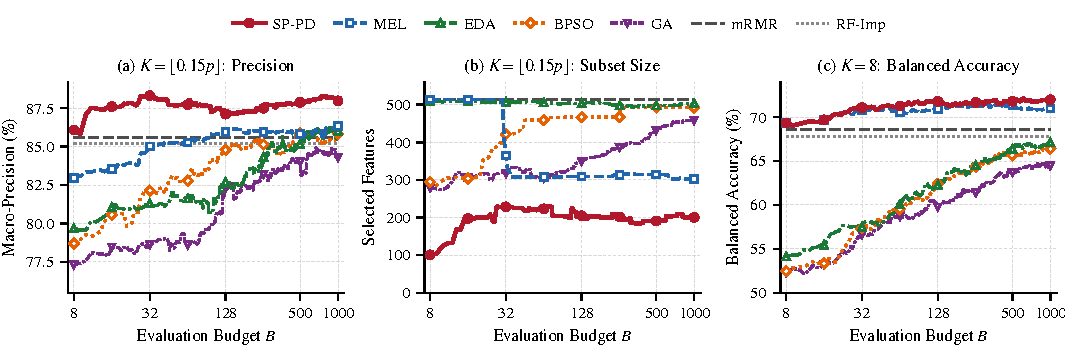
\includegraphics[width=\textwidth]{figures/fig1_highdim_convergence.pdf}
\caption{Convergence curves on high-dimensional benchmarks over $B \in [8, 1{,}000]$: (a) macro-precision, (b) subset size, and (c) balanced accuracy.}
\label{fig:highdim_conv}
\end{figure*}

As shown in Table~\ref{tab:highdim_wide} and Fig.~\ref{fig:highdim_conv}(b), SP-PD achieves these gains with the smallest subset size, selecting an average of 200.1 features at $K = \lfloor 0.15p \rfloor$. This represents a reduction of 33.9\% relative to MEL, 33.1\% relative to L1-LR, and 61.1\% relative to the filter baselines. While filters always saturate $K$ and GA, BPSO, and EDA expand to between 458 and 503 features, SP-PD identifies roughly 100 features by $B = 8$ and stabilizes near 200. On redundant datasets such as Gutenberg, malware, DLBCL/Lymphoma, and madelon, SP-PD removes over 85\% of candidate features without losing accuracy, as detailed in Appendix Table~\ref{tab:app_highdim_feat}.

At $K = \lfloor 0.15p \rfloor$, Table~\ref{tab:highdim_budgets} and Fig.~\ref{fig:highdim_conv}(a) show that SP-PD attains 87.12\% macro-precision at $B = 128$, already exceeding every baseline at $B = 1{,}000$, and significantly outperforms MEL by $B = 500$. Across all 23 groups at $K = 8$, the Friedman test confirms highly significant differences at every budget ($p < 1.3 \times 10^{-9}$). SP-PD ranks first across all budgets and metrics with a Friedman rank of 2.74, significantly surpassing all seven baselines other than MEL on macro-precision, BA, and macro-F1. In Fig.~\ref{fig:highdim_conv}(c), GA, BPSO, and EDA remain below static mRMR even at $B = 1{,}000$, and MEL peaks near $B = 256$ before declining to 70.99\% due to inner-validation overfitting. By contrast, SP-PD rises steadily to 71.98\%, maintaining advantages of 0.99 percentage points in BA and 0.83 percentage points in macro-F1 over MEL.

\begin{table*}[!t]
\centering
\begin{threeparttable}
\caption{Multi-Budget Results on High-Dimensional Benchmarks}
\label{tab:highdim_budgets}
\scriptsize
\setlength{\tabcolsep}{6.6pt}
\renewcommand{\arraystretch}{1.08}
\begin{tabular}{@{}lrrrr@{\hspace{18pt}}rrrrrr@{}}
\toprule
 & \multicolumn{4}{c}{$K = \lfloor 0.15p \rfloor$ (13 Groups)} & \multicolumn{6}{c}{$K = 8$ (23 Groups)} \\
\cmidrule(lr{18pt}){2-5} \cmidrule(l){6-11}
Algorithm & $B{=}128$ & $B{=}500$ & BA & F1 &
$B{=}128$ & $B{=}500$ & $B{=}1{,}000$ & BA & F1 & Rank \\
\midrule
GA      & 82.31\rlap{\textsuperscript{*}} & 84.02\rlap{\textsuperscript{*}} & 79.27 & 80.08\rlap{\textsuperscript{*}} & 65.60\rlap{\textsuperscript{*}} & 68.90\rlap{\textsuperscript{*}} & 69.99\rlap{\textsuperscript{*}} & 64.49\rlap{\textsuperscript{*}} & 63.90\rlap{\textsuperscript{*}} & 5.57 \\
BPSO    & 84.80 & 85.86 & 80.21 & 81.10 & 68.67\rlap{\textsuperscript{*}} & 72.12\rlap{\textsuperscript{*}} & 72.68\rlap{\textsuperscript{*}} & 66.38\rlap{\textsuperscript{*}} & 65.85\rlap{\textsuperscript{*}} & 4.83 \\
EDA     & 82.72 & 85.19 & 81.42 & 82.07\rlap{\textsuperscript{*}} & 67.49\rlap{\textsuperscript{*}} & 71.89\rlap{\textsuperscript{*}} & 72.48\rlap{\textsuperscript{*}} & 67.16\rlap{\textsuperscript{*}} & 66.94\rlap{\textsuperscript{*}} & 4.48 \\
MEL     & 85.95 & 85.83\rlap{\textsuperscript{*}} & 81.79 & 82.61\rlap{\textsuperscript{*}} & 76.47 & 76.39 & 76.19 & 70.99 & 71.63 & 3.30 \\
mRMR    & 85.58 & 85.58 & 81.27 & 81.99\rlap{\textsuperscript{*}} & 71.99\rlap{\textsuperscript{*}} & 71.99\rlap{\textsuperscript{*}} & 71.99\rlap{\textsuperscript{*}} & 68.59\rlap{\textsuperscript{*}} & 68.15\rlap{\textsuperscript{*}} & 4.43 \\
ReliefF & 84.60 & 84.60\rlap{\textsuperscript{*}} & 80.89 & 81.35\rlap{\textsuperscript{*}} & 60.36\rlap{\textsuperscript{*}} & 60.36\rlap{\textsuperscript{*}} & 60.36\rlap{\textsuperscript{*}} & 56.52\rlap{\textsuperscript{*}} & 53.83\rlap{\textsuperscript{*}} & 7.78 \\
L1-LR   & 83.88 & 83.88 & 80.88 & 81.27 & 66.90\rlap{\textsuperscript{*}} & 66.90\rlap{\textsuperscript{*}} & 66.90\rlap{\textsuperscript{*}} & 62.53\rlap{\textsuperscript{*}} & 61.34\rlap{\textsuperscript{*}} & 6.39 \\
RF-Imp  & 85.23\rlap{\textsuperscript{*}} & 85.23\rlap{\textsuperscript{*}} & 81.42 & 81.61\rlap{\textsuperscript{*}} & 71.22\rlap{\textsuperscript{*}} & 71.22\rlap{\textsuperscript{*}} & 71.22\rlap{\textsuperscript{*}} & 67.80\rlap{\textsuperscript{*}} & 67.64\rlap{\textsuperscript{*}} & 5.48 \\
\midrule
SP-PD   & \textbf{87.12} & \textbf{87.88} & \textbf{83.88} & \textbf{84.76} & \textbf{76.61} & \textbf{76.53} & \textbf{76.52} & \textbf{71.98} & \textbf{72.46} & \textbf{2.74} \\
\bottomrule
\end{tabular}
\begin{tablenotes}[flushleft]
\scriptsize
\item Budget columns report mean macro-precision (\%); BA, F1, and Friedman Rank are evaluated at $B = 1{,}000$.
\item[*] SP-PD significantly outperforms the comparison algorithm (Wilcoxon signed-rank test, $\alpha = 0.05$).
\end{tablenotes}
\end{threeparttable}
\end{table*}

